In order to asses to what extent using {\em Umbra Designer} improves the productivity of service development,
we have performed an experiment consisting in the construction of ten services of varying complexity using the 
graphical tool, and the comparison with the effort to develop the same services using directly the framework API
(i.e. programming directly in Java). 

We had two participants in our experiment, both last year undergraduates in Computer Science. The first
participant had some knowledge of telecommunications services, but no deep knowledge of the {\em Umbra 
framework}'s API. The second participant had some 5 months of experience using the API. 
Each participant built 5 services using the tool and 5 different ones using the API.
Each service was built in a different session, on a different day. The participants were given enough time
to read each service description and think a solution. When they were ready, we measured the time they
employed to implement the solution, one using the graphical tool and the other using directly the Java API. 
This way, we leave out effects related to problem understanding and solution design, and strictly measure
service production efficiency by two different means.

The services used in the experiment varied in complexity, ranging from simple ones (five states
%, including initial and final, 
and few transitions) to medium size (more than 15 states and 35 transitions). In each session, the participants 
were given textual definitions of the service to be developed in the session. As an example, the description of one 
of the services was the following: ``{\em Build a voice service for a computer repair shop. The service will play a 
message, and then, it will solicit the year in which the computer was bought. The user should type the solicited 
year using the telephone keyboard. Then, if the computer is still in the guarantee period (2 years), the service 
will solicit the serial number and the address, which will get recorded}''. 
Fig.~\ref{fig:repairingService} shows the service finally built for the previous service definition, 
using the graphical tool. The Properties view contains the configuration of the actions in the transition
entering state {\em SolicitarDireccion} ({\em Solicit Address}). The transition has two actions, one for recording
the address (whose configuration is shown), and the other one is just one line of Java code to transform the 
different key strokes into a String service variable (not shown).

\figeps{repairingService}{0.3}{Service \#7: a simple service for a computer shop.}

Other services built include a game for guessing a number, a time service which informs of the current time, 
a taxi call service, a simplified airport information service and a service for pizza ordering (see Table~\ref{tab:results}).

Table~\ref{tab:results} summarizes the experiment results. The columns show: (1) the name of the service;
(2--5) the size of its model-based solution (number of states and transitions, cyclomatic complexity and lines of extra 
Java code in {\em JavaCode} actions); (6--7) the number of source lines of code (SLOC, not 
counting blank lines or comments) of the service that are generated by the tool or hand-coded using the API; (8--9) 
the minutes taken to build the service using the tool and the API; and (10) the efficiency gain when using the tool 
compared to using the API (minutes and percentage). In the case of using the API, the measurements also include 
the creation time of additional artefacts, like property files, needed to deploy the service (but automatically generated by the tool).

\begin{table}[h]
\centering
\scriptsize
\begin{tabular}{|p{0.7cm}p{2.0cm}||p{0.9cm}|p{0.9cm}|p{0.9cm}|p{0.9cm}||p{0.8cm}|p{0.8cm}||p{0.8cm}|p{0.8cm}||p{1.5cm}|}
\hline
&        		& \multicolumn{4}{|c||}{{\bf Model Size}} & \multicolumn{2}{|c||}{{\bf SLOC}} & \multicolumn{2}{|c||}{{\bf Time (min.)}}  & \\ \hline
&        		& States & Trans.  & Cycles & Java Extra & Tool & API                                     & Tool & API                            & {\bf Gain (min./\%)} \\ \hline
\#1 : & Message + Key  & 5        & 6         & 3        & 0 & 383 & 395 & 7                    &  30            & {\bf 23 (76\%)} \\ \hline
\#2 : & Taxi Call           & 8        & 10       & 4        & 2 & 441 & 403 & 9                    &  21              & {\bf 12 (57\%)} \\ \hline
\#3 : & Guessing Game & 8        & 13       & 6        & 3 & 448 & 415 & 23                  &  42            & {\bf 19 (45\%)} \\ \hline
\#4 : & Postal Code/ Time Warning & 6        & 12       & 8        & 12 & 439 & 453 & 30 &  53          & {\bf 23 (43\%)} \\ \hline
\#5 : & Traffic              & 9      & 12         & 5      & 4 & 450 & 453 & 20                  &  35              &  {\bf 15  (42\%)} \\ \hline
\#6 : & Survey             & 10      & 14       & 6        & 0  & 529 & 477 & 15                  &  33            & {\bf 18 (54\%)} \\ \hline
\#7 : & Computer Shop & 9       & 13         & 6        & 4 & 493 & 501 & 20                  &  40             &  {\bf 20 (50\%)} \\ \hline
\#8 : & Airport             & 11      & 23         & 14      & 8 & 542 & 514 & 60                  &  90             & {\bf 30  (33\%)} \\ \hline
\#9 : & Time Service    & 5        & 4         & 1        & 269 & 640 & 749 & 24                  &  36             & {\bf 12 (33\%)} \\ \hline
\#10 : & Pizza Orders   & 17     & 52         & 37      & 60 & 963 & 925 & 150                &  200            & {\bf 50 (25\%)} \\ \hline
\end{tabular}
\caption{Evaluation of the construction of several services.}
\label{tab:results}
\end{table}
%\#7 : & Simple Message & 6                  &  15           & 7        & 10         & 5        & 2           & 16         & 949 \\ \hline

The experiments show good correlation between the number of SLOC of the hand-coded solution and of the code generated by the tool. 
Regarding productivity, by using the tool we observe an increase of around 45\% in the average case. In all cases, 
the time to develop a service with the tool
was less than using the API directly. Fig.~\ref{fig:graphics}(a) shows a graphic showing the net gain with respect to service size (SLOC
of the hand-coded solution), 
while the right shows the percentage gain with respect to size. The graphic shows higher percentual gains for smaller services; however, the highest net gain was with the 
largest service. We noted higher gains in cases were the service accommodated well the abstractions of state machines: few cycles, few decision
nodes, and few extra lines of code.

\begin{figure}[h!tb]
  \centering
    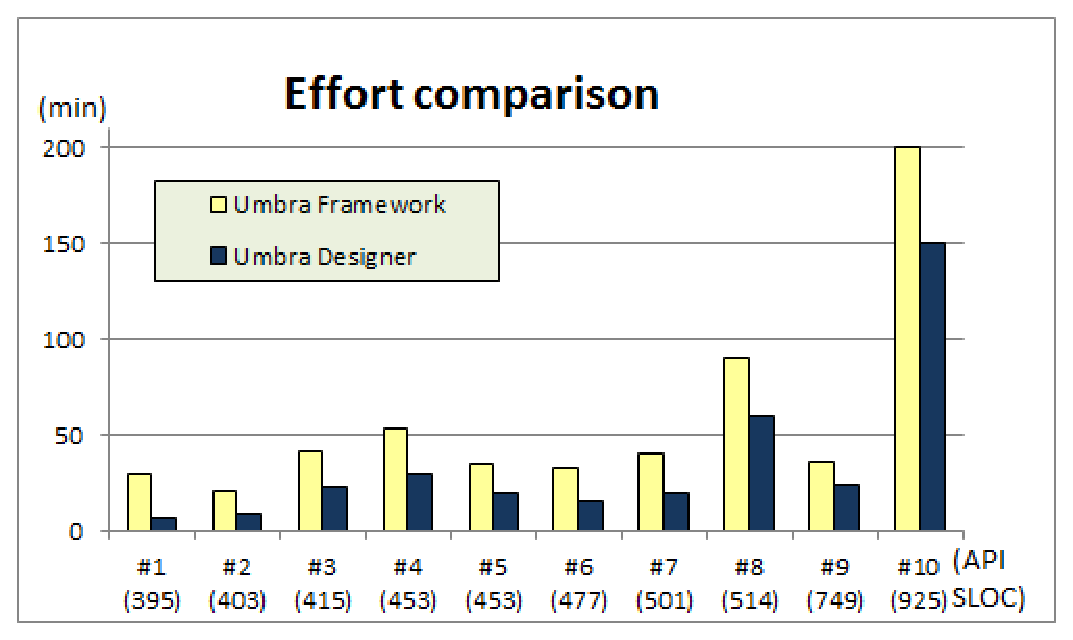
\includegraphics[scale = 0.35]{figures/effort.eps} %\caption{A figure \label{fig:figure}}
  \hspace{0.1cm}
    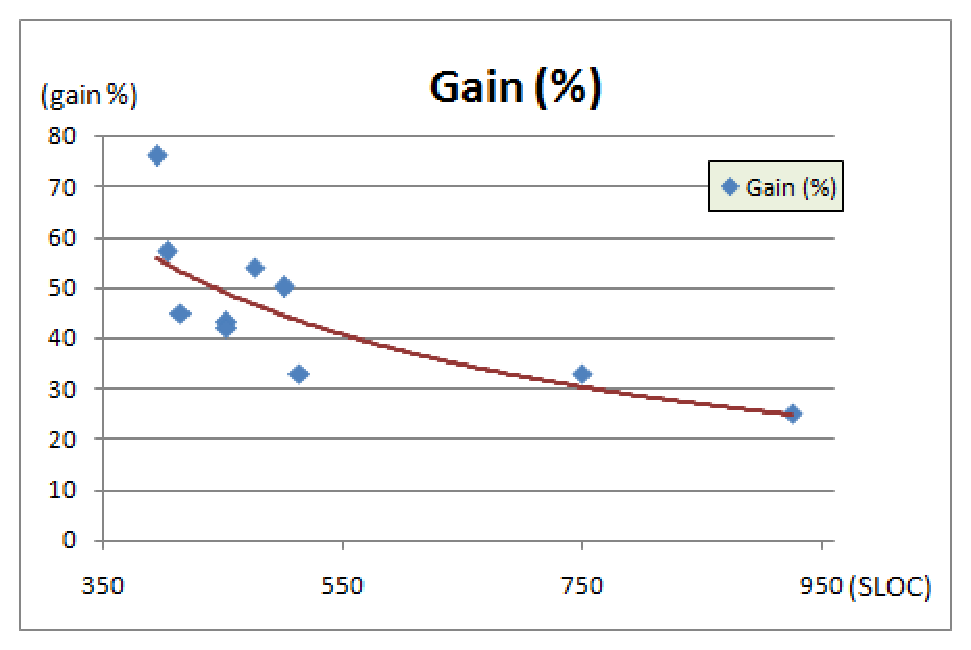
\includegraphics[scale = 0.35]{figures/gain.eps} %\caption{Another figure \label{fig:another}}
  \caption{Development effort comparison (left). Efficiency gain (right).}
  \label{fig:graphics}
\end{figure}

Altogether, the experiment shows benefits in efficiency when using the graphical tool. Moreover, we believe that it provides further benefits 
concerning: built-in validation checks, maintainability, understandability and reutilization of services. Experiments to assess these properties are 
subject to future work. As a preliminary result, we experienced in measuring the effort gain in maintainability, where a modification to service \#1 
consisting in the introduction of an error message on certain events was introduced. In this case, using the graphical tool led to shorter times 
(6 minutes vs 15 minutes). A finding related to this issue was that both participants found useful to draw state machine-like diagrams on paper, 
as a design sketch, before starting coding using the API. This means that the graphical model was deemed a good abstraction to describe services.